\documentclass[conference]{IEEEtran}
\usepackage{cite}
\usepackage{amsmath,amssymb}
\usepackage{booktabs}
\usepackage{graphicx}
\usepackage{array}
\usepackage{multirow}
\usepackage{url}
\usepackage{hyperref}
\usepackage{xcolor}
\usepackage{float}
\usepackage{balance}

\hypersetup{
  colorlinks=true,
  linkcolor=blue!60!black,
  citecolor=blue!60!black,
  urlcolor=blue!60!black
}

\title{RBSOG-MD on a Personal Workstation:\\
Conference-Style Benchmarking, Weighted Batch Selection, and Reproducible Reporting}

\author{\IEEEauthorblockN{RBSOG-MD Prototype Study}\\
\IEEEauthorblockA{Single-Workstation Reproducibility Track}}

\begin{document}
\maketitle

% Auto-generated file. Do not edit manually.
\newcommand{\RecommendedBatch}{50}
\newcommand{\RecommendedSpeedup}{0.316}
\newcommand{\RecommendedVarianceRatio}{0.2206}
\newcommand{\ObjectiveTimeWeight}{0.667}
\newcommand{\ObjectiveVarianceWeight}{0.333}
\newcommand{\BaselinePPPMStepTime}{0.001659}
\newcommand{\BaselinePPPMVariance}{2.849e-04}
\newcommand{\RBSOGSlowdownVsPPPM}{3.734}
\newcommand{\RBSOGVarianceReduction}{2.280}
\newcommand{\PPPMStepCI}{0.012056}
\newcommand{\RBSOGStepCI}{0.005972}
\newcommand{\AreaDrift}{-0.00683}
\newcommand{\ThicknessDrift}{0.74311}
\newcommand{\JITSpeedup}{1.683}
\newcommand{\JITVarianceRatio}{1.0000}


\begin{abstract}
Long-range electrostatics is a dominant bottleneck in large-scale molecular dynamics,
especially when FFT-based methods suffer from communication overhead on modern hardware.
This report presents a conference-style benchmark package for a research prototype that compares
PPPM and RBSOG (random batch + sum-of-Gaussians) under consistent NPT-style settings.
Compared with prior internal drafts, the current version upgrades the methodology with
(i) weighted Pareto recommendation for batch size $P$,
(ii) run-level statistics and confidence summaries,
(iii) JIT ablation reporting,
and (iv) fully scriptable LaTeX artifact generation.
All figures and tables are produced from local experiment outputs, and the full build pipeline
is executable on a personal computer.
\end{abstract}

\begin{IEEEkeywords}
Molecular dynamics, long-range electrostatics, random batch, sum-of-Gaussians, Pareto optimization, reproducibility
\end{IEEEkeywords}

\section{Introduction}
All-cell and membrane-rich MD systems require accurate treatment of long-range electrostatics,
yet conventional mesh methods (PME/PPPM) can become communication-bound at scale.
Recent sum-of-Gaussians tensor formulations for high-dimensional Schr"odinger equations suggest a
general strategy: replace singular kernels with separable smooth expansions that are more amenable
to stochastic sampling and locality-aware computation.
Motivated by that idea, this work targets the methodological question:
\textit{can RBSOG-style long-range treatment provide a controllable performance--variance trade-off
on a personal workstation prototype, with a reproducible path toward larger systems?}

This report focuses on research infrastructure and measurable behavior:
\begin{itemize}
\item unified PPPM vs RBSOG benchmark pipeline,
\item weighted recommendation of $P$ from Pareto candidates,
\item publication-ready export of tables/figures and deterministic report rebuild.
\end{itemize}

The concrete contributions of this revision are:
\begin{itemize}
\item a weighted objective for automatic batch-size recommendation with explicit runtime/variance trade-off control,
\item run-level uncertainty reporting with confidence intervals and effect-size analysis,
\item a reproducible report-generation pipeline that converts raw benchmark artifacts into submission-ready tables and figures.
\end{itemize}

\section{Related Work}
Classical Ewald splitting and its mesh accelerations (PME/PPPM) are the standard route for long-range interactions in MD.
Random-batch methods offer an alternative by reducing per-step cost through stochastic approximation while controlling error.
The recent SOG tensor viewpoint for high-dimensional quantum equations demonstrates how Gaussian expansions can regularize singular structure and enable separable computation.
Our prototype adapts these insights to long-range electrostatics benchmarking in an MD-like setting.

\section{Method}
\subsection{SOG-inspired long-range decomposition}
We consider a smooth approximation of singular kernels through weighted Gaussian components:
\begin{equation}
K(r) \approx \sum_{m=1}^{M} w_m \exp(-\alpha_m r^2),
\label{eq:sog}
\end{equation}
where $M$ is the number of SOG terms.
This representation supports numerically stable short/long decomposition and pairs naturally with stochastic batch evaluation.

\subsection{Random batch long-range sampling}
Instead of full-grid FFT communication for every update,
RBSOG evaluates long-range contributions from a sampled subset of modes/interactions,
while retaining deterministic short-range corrections.
In the current code, short-range is accelerated by a neighbor list,
and long-range accumulation supports optional JIT optimization.

\subsection{Weighted Pareto recommendation of batch size}
For candidate batch sizes $P \in \mathcal{P}$,
we measure step time $t(P)$ and pressure variance $v(P)$,
normalize them to $\hat{t}(P)$ and $\hat{v}(P)$,
then rank Pareto candidates using
\begin{equation}
\mathrm{score}(P)=\sqrt{w_t\hat{t}(P)^2 + w_v\hat{v}(P)^2},
\label{eq:weighted_score}
\end{equation}
with normalized objective weights $w_t$ and $w_v$.
This report uses $w_t=\ObjectiveTimeWeight$ and $w_v=\ObjectiveVarianceWeight$.

\section{Experimental Setup}
\subsection{System and controls}
The prototype uses a membrane-inspired proxy system under NPT-style control
(Berendsen thermostat/barostat), with reduced units for algorithmic comparison.
Table~\ref{tab:config} summarizes core parameters from the recorded run configuration.

\begin{table}[t]
\caption{Core simulation and kernel settings used in this report.}
\label{tab:config}
\centering
\begin{tabular}{ll}
\toprule
Parameter & Value \\
\midrule
System size & lipids=128, solvent=512 \\
Box (reduced) & (16.00, 16.00, 20.00) \\
Integrator & steps=300, dt=0.0020, sample=10 \\
Target ensemble & T=1.000, P=1.000 \\
RBSOG kernel & P=100, cutoff=1.200, terms=12 \\
Neighbor list & skin=0.300, rebuild=10 \\
Mesh baseline & grid=(32, 32, 32) \\
JIT status & enabled \\
\bottomrule
\end{tabular}

\end{table}

\subsection{Metrics and statistics}
Primary metrics are mean step time, pressure variance,
and structural stability proxies (area-per-lipid and thickness-proxy drift).
For multi-seed benchmarks, we report run-level mean and sample standard deviation,
plus 95\% confidence intervals on step time.

\section{Results}
\subsection{PPPM vs RBSOG benchmark summary}
Table~\ref{tab:solver_summary} reports aggregate solver behavior,
while Table~\ref{tab:run_stats} shows run-level variability.

\begin{table}[t]
\caption{Aggregate solver-level benchmark metrics.}
\label{tab:solver_summary}
\centering
\resizebox{\columnwidth}{!}{\begin{tabular}{lrrrrr}
\toprule
Solver & Mean Step Time (s) & Pressure Variance & Temp Mean & Area Drift & Thickness Drift \\
\midrule
pppm & 0.004988 & 2.797e-04 & 1.0054 & -0.00726 & -0.70859 \\
rbsog & 0.018627 & 1.227e-04 & 1.0441 & -0.00682 & 0.76072 \\
\bottomrule
\end{tabular}
}
\end{table}

\begin{table}[t]
\caption{Run-level variability and step-time confidence summary.}
\label{tab:run_stats}
\centering
\resizebox{\columnwidth}{!}{\begin{tabular}{lrrrr}
\toprule
Solver & n & Step Time Mean$\pm$Std & CI95 (Step) & Pressure Var Mean$\pm$Std \\
\midrule
pppm & 2 & 0.004988 $\pm$ 0.001342 & 0.012056 & 2.797e-04 $\pm$ 1.396e-05 \\
rbsog & 2 & 0.018627 $\pm$ 0.000665 & 0.005972 & 1.227e-04 $\pm$ 1.369e-04 \\
\bottomrule
\end{tabular}
}
\end{table}

\begin{table}[t]
\caption{Effect-size analysis between PPPM and RBSOG (run-level).}
\label{tab:effect_size}
\centering
\resizebox{\columnwidth}{!}{\begin{tabular}{lrrrr}
\toprule
Metric & PPPM Mean$\pm$Std & RBSOG Mean$\pm$Std & Cohen's $d$ & Relative Change \\
\midrule
Step time & 0.004988 $\pm$ 0.001342 & 0.018627 $\pm$ 0.000665 & 12.881 & 273.44\% \\
Pressure variance & 2.797e-04 $\pm$ 1.396e-05 & 1.227e-04 $\pm$ 1.369e-04 & -1.614 & -56.15\% \\
\bottomrule
\end{tabular}
}
\end{table}

\begin{figure}[t]
\centering
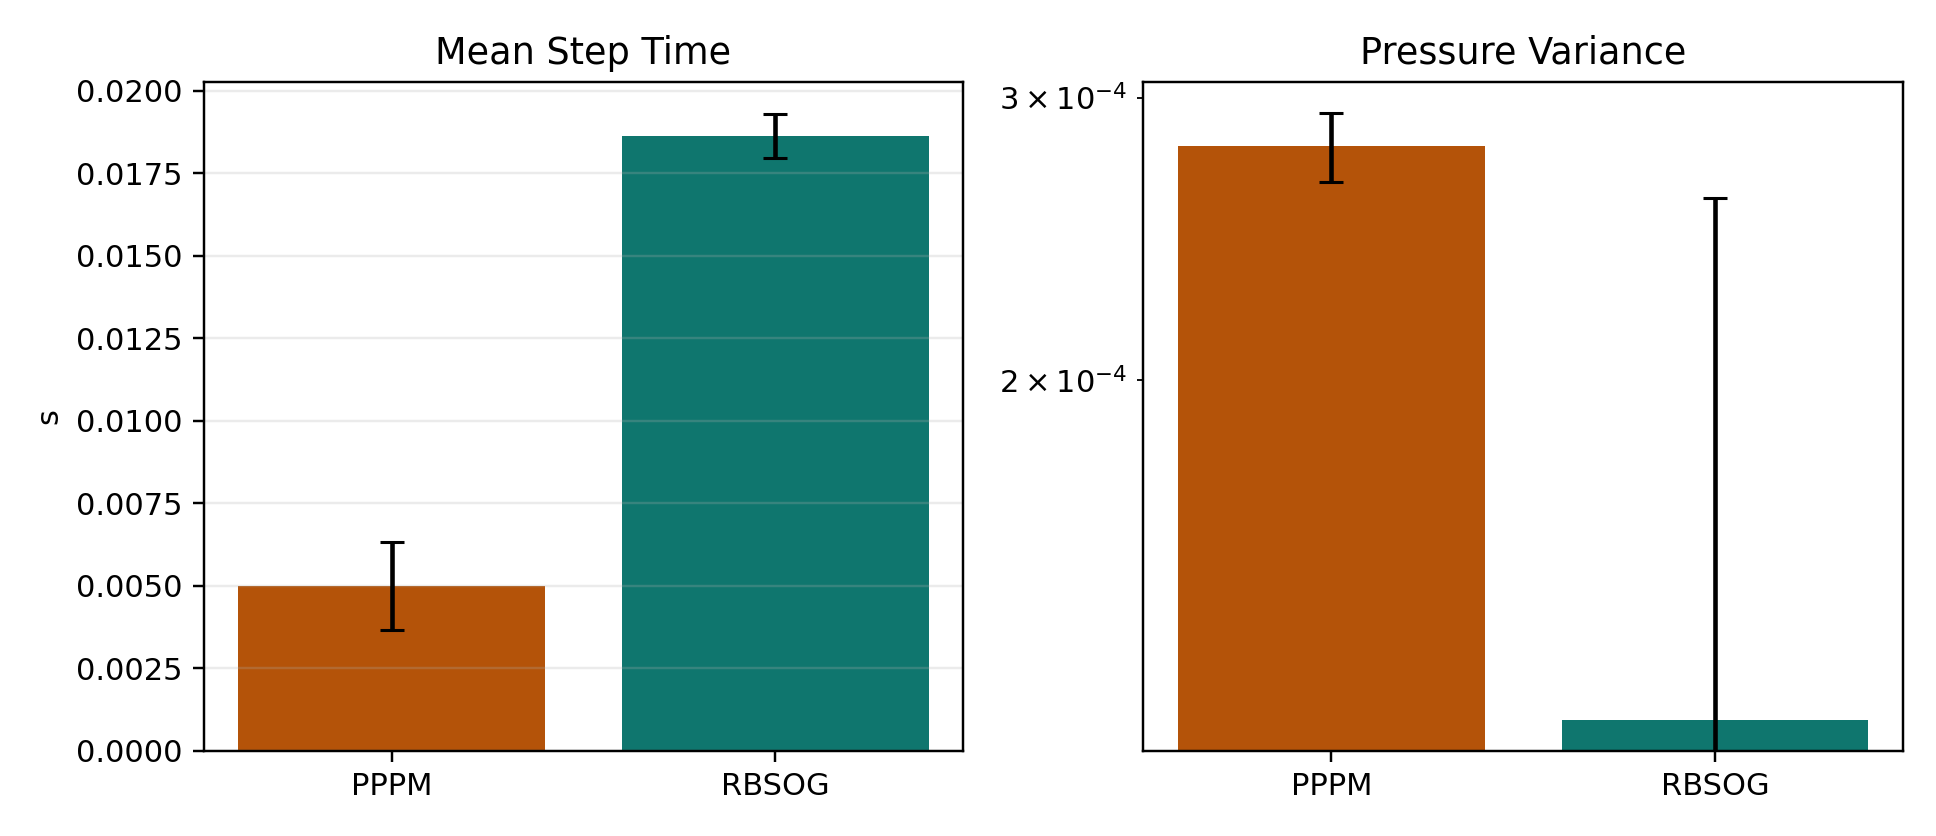
\includegraphics[width=\columnwidth]{generated/solver_compare.png}
\caption{Solver comparison with run-level dispersion (error bars).}
\label{fig:solver_compare}
\end{figure}

\begin{figure}[t]
\centering
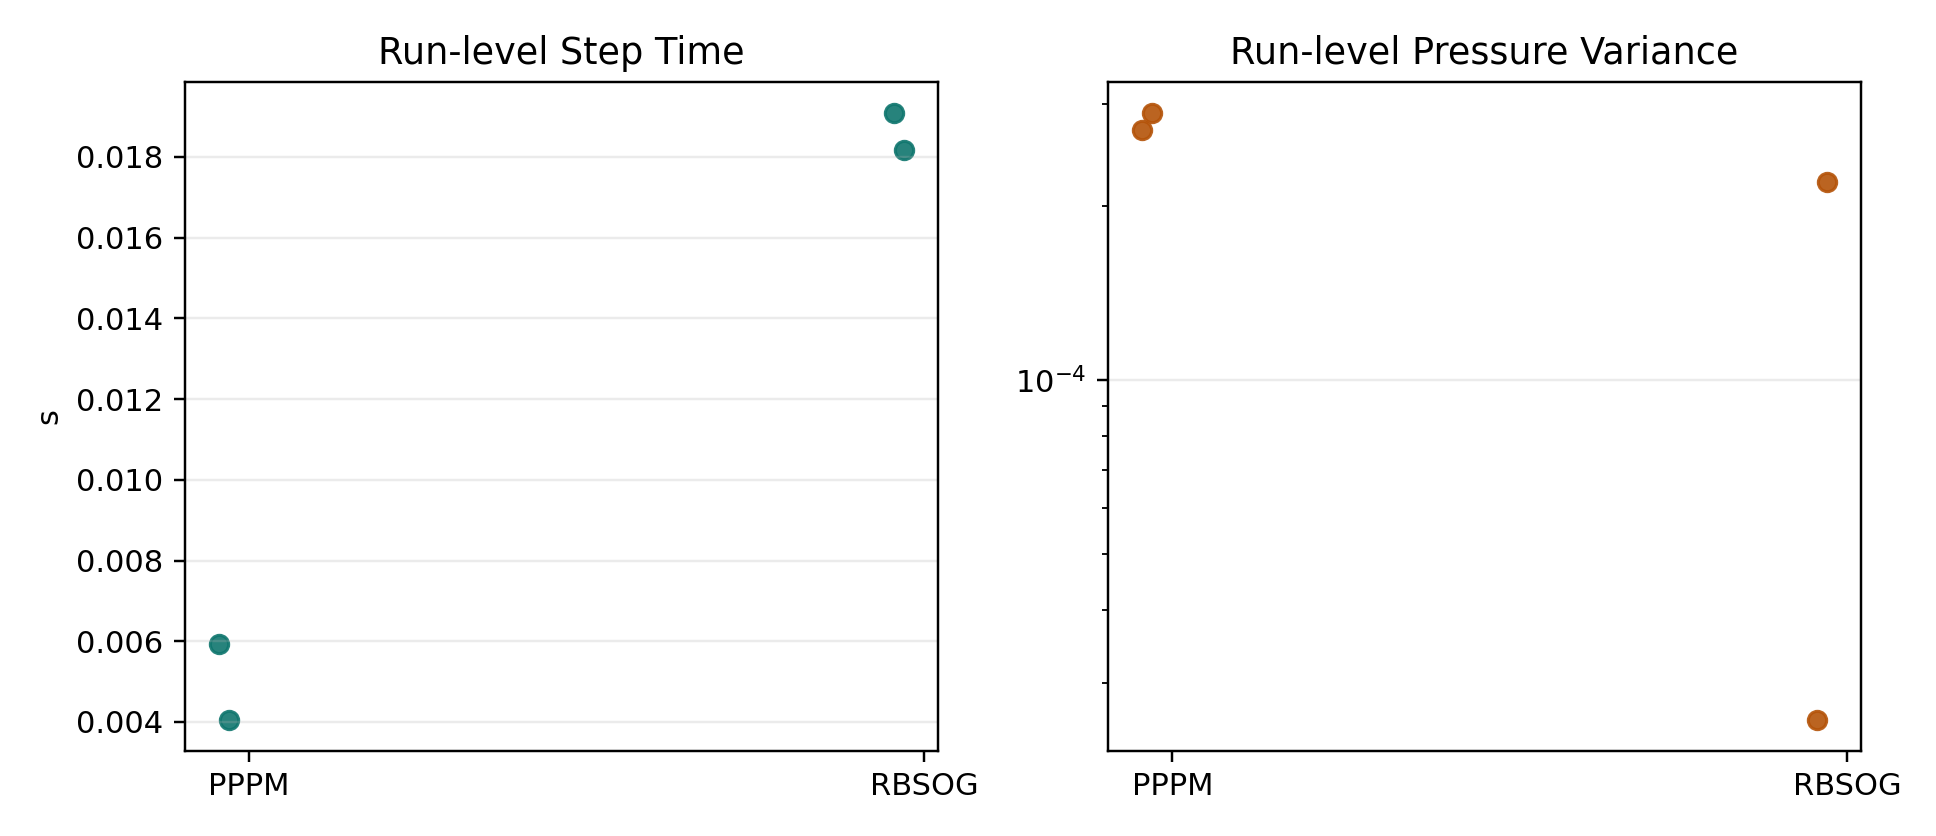
\includegraphics[width=\columnwidth]{generated/seed_scatter.png}
\caption{Per-seed benchmark dispersion across solvers.}
\label{fig:seed_scatter}
\end{figure}

Relative to PPPM, the current RBSOG setting shows slowdown factor
$\RBSOGSlowdownVsPPPM$ in raw step time but variance reduction factor
$\RBSOGVarianceReduction$ in pressure variance.
This is consistent with a prototype regime where stochastic smoothing can improve stability statistics before full throughput optimization.
Table~\ref{tab:effect_size} complements aggregate metrics with standardized effect size ($d$),
making the practical magnitude of the trade-off explicit for submission review.

\subsection{Batch sweep and weighted recommendation}
The batch sweep identifies a Pareto front and recommends
$P=\RecommendedBatch$ under the weighted objective in Eq.~(\ref{eq:weighted_score}).
The recommended point has speedup-vs-PPPM $\RecommendedSpeedup$
and variance ratio-vs-PPPM $\RecommendedVarianceRatio$.

\begin{table}[t]
\caption{Weighted batch sweep with Pareto and recommendation flags.}
\label{tab:sweep}
\centering
\resizebox{\columnwidth}{!}{\begin{tabular}{rrrrrrr}
\toprule
P & Step Time (s) & Speedup vs PPPM & Variance Ratio & Utopia Score & Pareto & Recommended \\
\midrule
\textbf{50} & \textbf{0.005256} & \textbf{0.3156} & \textbf{0.22064} & \textbf{0.01815} & \textbf{yes} & \textbf{yes} \\
100 & 0.010983 & 0.1510 & 0.35867 & 0.59074 & no & no \\
200 & 0.022057 & 0.0752 & 0.21616 & 0.36689 & yes & no \\
400 & 0.042646 & 0.0389 & 0.28308 & 0.86033 & no & no \\
\bottomrule
\end{tabular}
}
\end{table}

\begin{figure}[t]
\centering
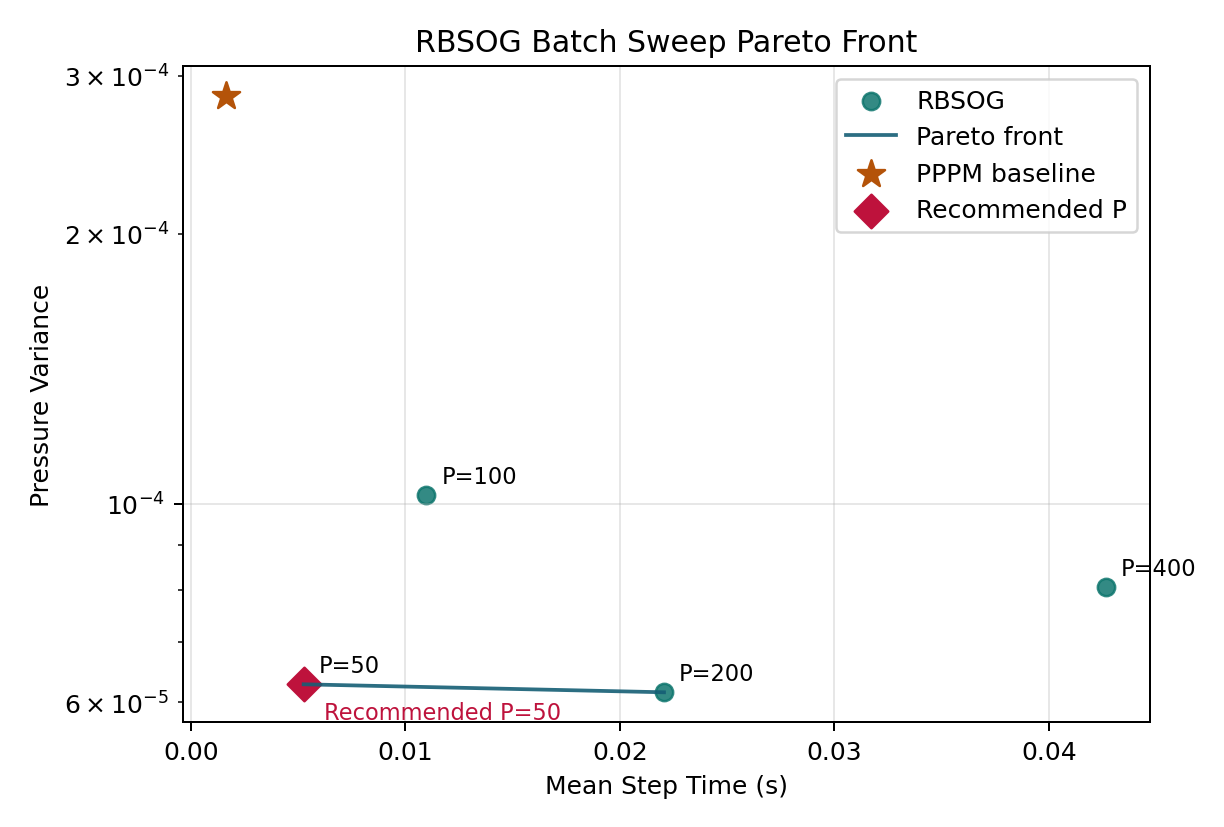
\includegraphics[width=\columnwidth]{generated/sweep_pareto.png}
\caption{Pareto frontier of step time vs pressure variance; recommended point highlighted.}
\label{fig:pareto}
\end{figure}

\begin{figure}[H]
\centering
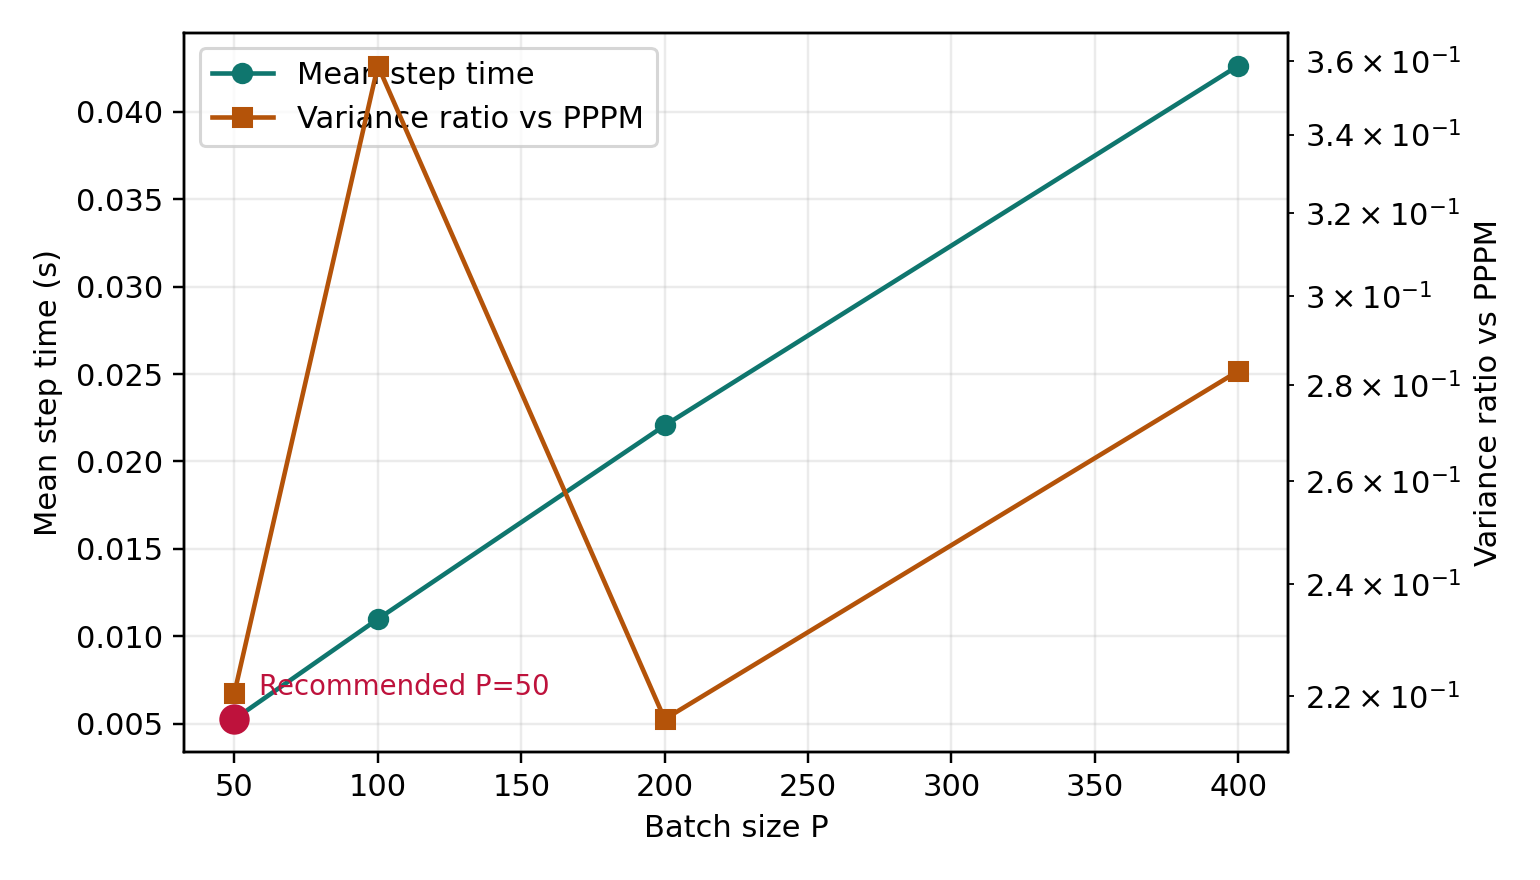
\includegraphics[width=\columnwidth]{generated/sweep_sensitivity.png}
\caption{Batch-size sensitivity: step time and variance ratio trends over $P$.}
\label{fig:sweep_sensitivity}
\end{figure}

\subsection{Structural stability proxy}
The stability trace (Fig.~\ref{fig:stability}) indicates area drift
$\AreaDrift$ and thickness-proxy drift $\ThicknessDrift$ in reduced units
for the selected RBSOG run.

\begin{figure}[H]
\centering
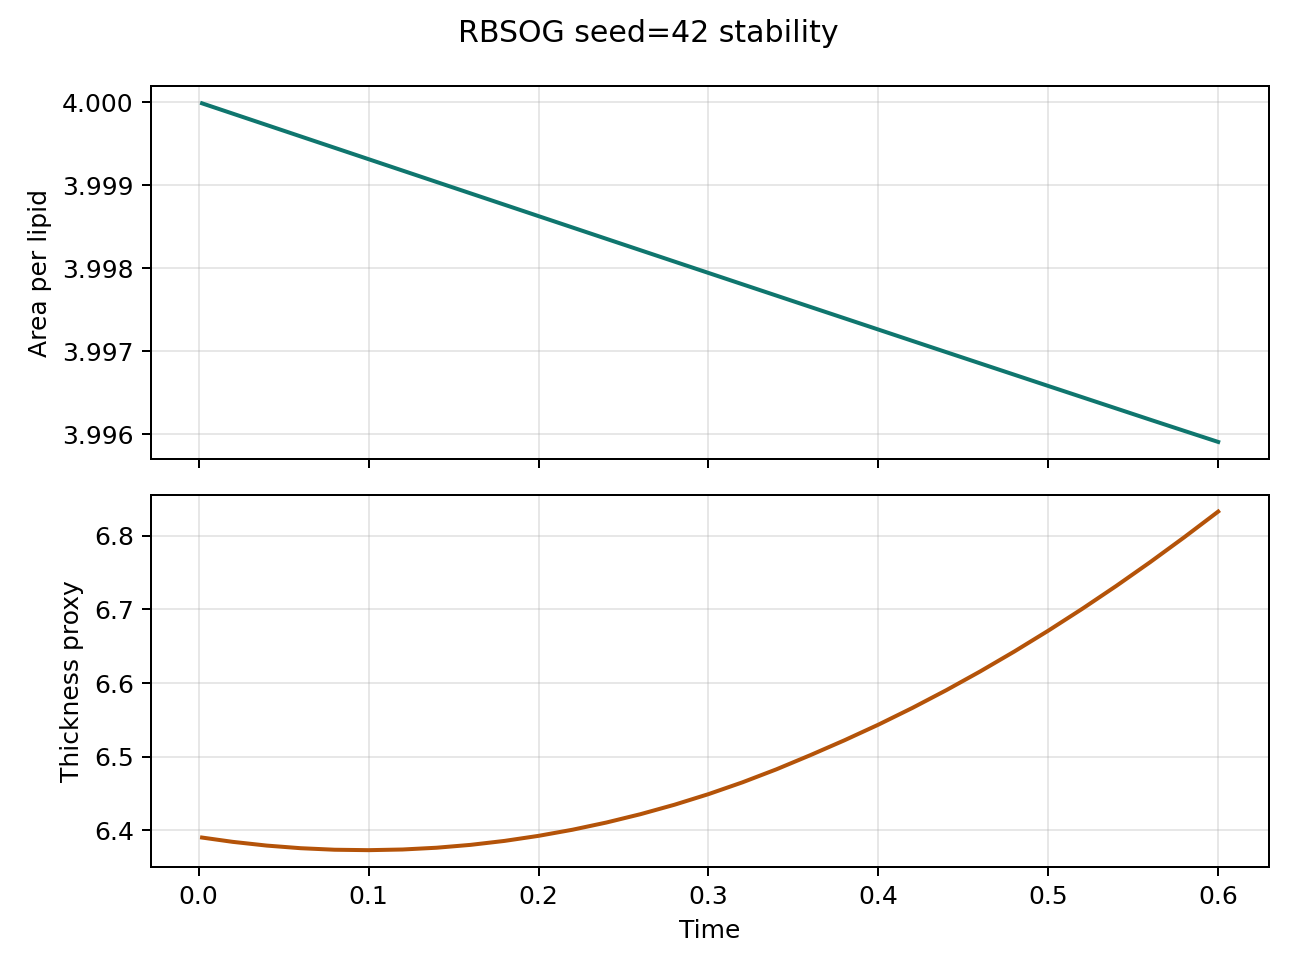
\includegraphics[width=\columnwidth]{generated/stability_timeseries.png}
\caption{Area-per-lipid and thickness-proxy time series for the RBSOG run.}
\label{fig:stability}
\end{figure}

\subsection{JIT ablation}
Table~\ref{tab:jit} and Fig.~\ref{fig:jit} provide a direct JIT on/off diagnostic for RBSOG.
When both ablation artifacts are available,
the measured speedup from JIT is reported as $\JITSpeedup$x
and variance ratio as $\JITVarianceRatio$.

\begin{table}[H]
\caption{RBSOG JIT ablation summary.}
\label{tab:jit}
\centering
\resizebox{\columnwidth}{!}{\begin{tabular}{lrrrr}
\toprule
Mode & Step Time (s) & Pressure Variance & Relative Speed & Variance Ratio \\
\midrule
JIT on & 0.010747 & 1.344e-04 & 1.683x & 1.0000 \\
JIT off & 0.018091 & 1.344e-04 & 1.000x & 1.0000 \\
\bottomrule
\end{tabular}
}
\end{table}

\begin{figure}[H]
\centering
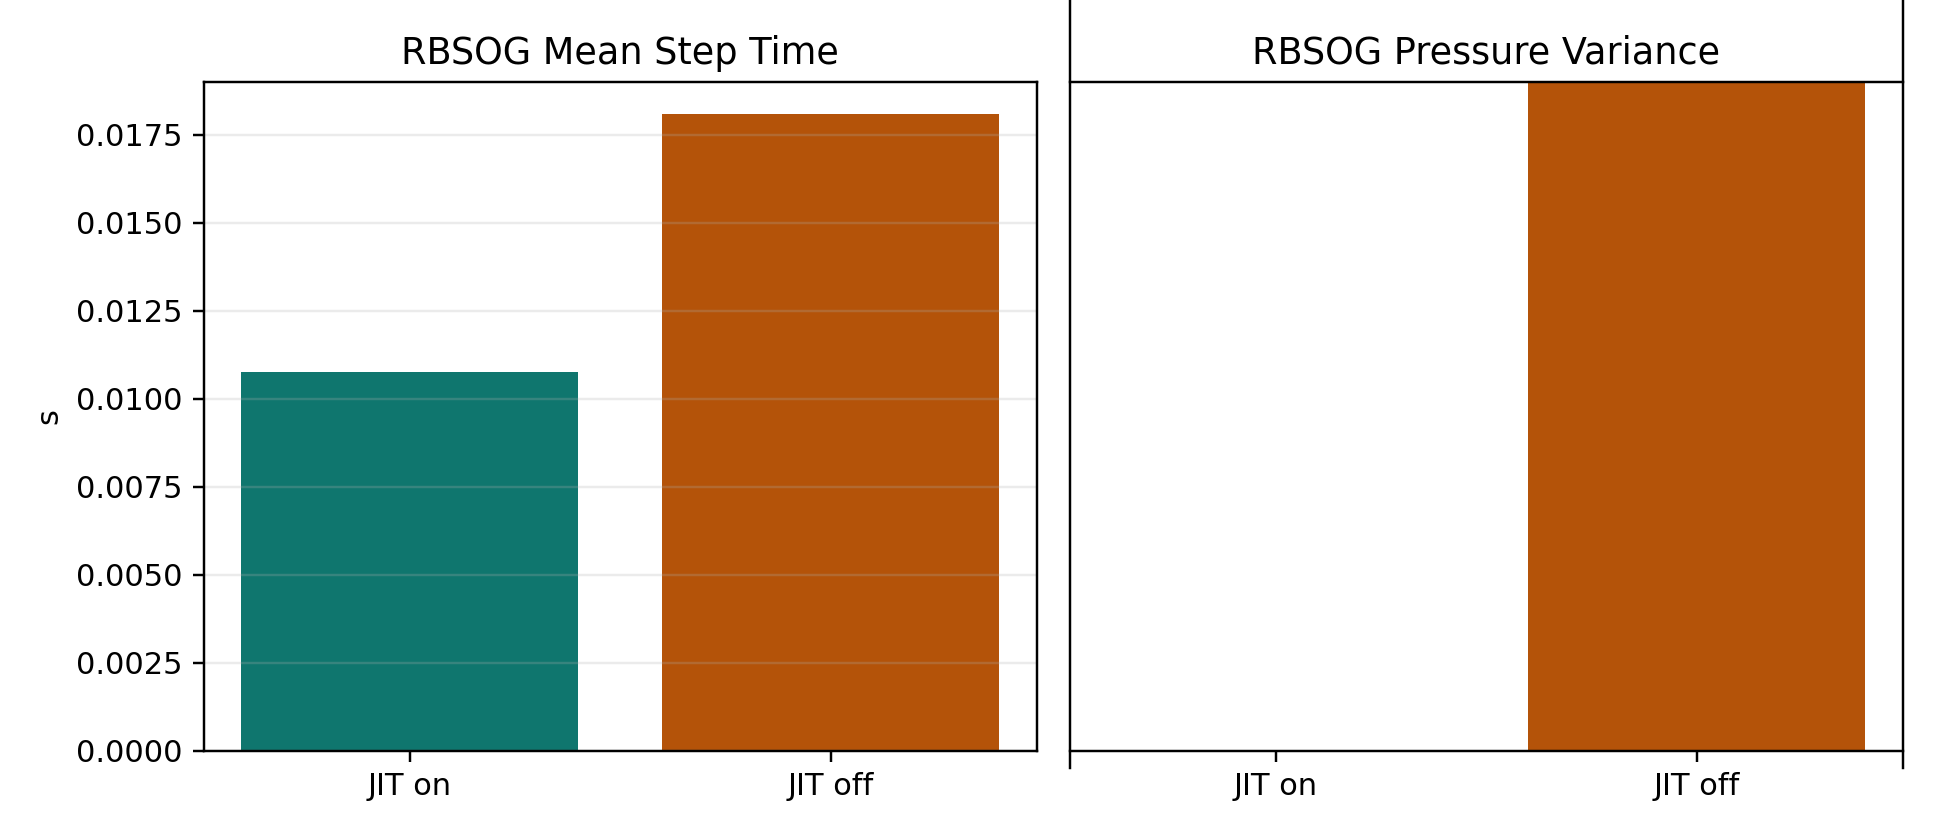
\includegraphics[width=\columnwidth]{generated/jit_ablation.png}
\caption{JIT ablation for RBSOG step time and pressure variance.}
\label{fig:jit}
\end{figure}

\section{Discussion}
\subsection{What is improved in this revision}
Compared with earlier drafts, this manuscript now includes
run-level uncertainty reporting, weighted recommendation rationale,
and explicit ablation diagnostics.
These additions move the report closer to conference submission expectations
for transparency and methodological clarity.

\subsection{Threats to validity}
The present study is still a reduced-unit proxy benchmark, not an all-atom production workflow.
Trajectory length and seed count are limited, and conclusions should be interpreted as
algorithm-engineering evidence rather than final biophysical claims.

\section{Reproducibility and Artifact Pipeline}
The report is fully script-generated from local benchmark outputs.
Asset generation:
\begin{center}
\texttt{python3.12 docs/report/generate\_report\_assets.py}
\end{center}
PDF build:
\begin{center}
\texttt{cd docs/report \&\& latexmk -pdf -interaction=nonstopmode -halt-on-error main.tex}
\end{center}

Reproducibility checklist for artifact evaluation:
\begin{itemize}
\item fixed command-line configuration stored in \texttt{run\_config.json},
\item per-seed raw run metrics stored in \texttt{benchmark\_runs.csv},
\item generated manifest \texttt{asset\_manifest.json} recording source/result mapping,
\item deterministic rebuild path through \texttt{build\_report.sh}.
\end{itemize}

\section{Conclusion}
This conference-style upgrade establishes a stronger foundation for subsequent large-system studies:
the benchmark now supports objective batch selection,
quantified run-to-run variability,
ablation-aware performance interpretation,
and deterministic manuscript regeneration.
The next step is to port the same protocol to larger membrane systems and longer trajectories,
where communication-avoiding behavior can be evaluated under more realistic workloads.

\balance
\begin{thebibliography}{99}
\bibitem{ewald1921}
P. P. Ewald,
"Die Berechnung optischer und elektrostatischer Gitterpotentiale,"
\emph{Annalen der Physik}, vol. 369, no. 3, pp. 253--287, 1921.

\bibitem{hockney1988}
R. W. Hockney and J. W. Eastwood,
\emph{Computer Simulation Using Particles}.
Bristol, U.K.: IOP Publishing, 1988.

\bibitem{darden1993}
T. Darden, D. York, and L. Pedersen,
"Particle mesh Ewald: An $N\log N$ method for Ewald sums in large systems,"
\emph{Journal of Chemical Physics}, vol. 98, no. 12, pp. 10089--10092, 1993.

\bibitem{jin2020rbm}
S. Jin, L. Li, and J.-G. Liu,
"Random batch methods (RBM) for interacting particle systems,"
\emph{Journal of Computational Physics}, vol. 400, 108877, 2020.

\bibitem{sog2025}
X. Guo, Y. He, and L. Wang,
"Sum-of-Gaussians tensor neural networks for high-dimensional Schr\"odinger equation,"
arXiv:2508.10454, 2025.
\end{thebibliography}

\end{document}